\capitulo{4}{Técnicas y herramientas}

En esta sección se presentan las técnicas y herramientas fundamentales empleadas en el desarrollo del proyecto. A continuación, se presentan las tecnicas empleadas durante el desarrollo del proyecto.
\section{Técnicas}
\subsection {\textit{Scrum}}

La metodología ágil \textit{Scrum}~\cite{scrum-guide} es un marco de trabajo muy extendido en el ámbito del desarrollo de software, especialmente útil en proyectos donde los requisitos pueden variar con frecuencia o no están completamente definidos desde el inicio. Su principal objetivo es facilitar una entrega continua de valor al cliente mediante un proceso iterativo e incremental.

\textit{Scrum} promueve la colaboración activa entre todos los miembros del equipo, fomenta la transparencia en cada fase del desarrollo y permite una adaptación rápida a cambios en las necesidades o prioridades. El trabajo se estructura en ciclos cortos llamados \textit{sprints}, cuya duración habitual oscila entre una y cuatro semanas. Cada \textit{sprint} comienza con una sesión de planificación (\textit{sprint planning}), seguida de reuniones breves diarias (\textit{daily stand-up}) para monitorizar el progreso (no realizadas en este proyecto), y finaliza con una revisión del trabajo desarrollado (\textit{sprint review}) y una retrospectiva orientada a detectar oportunidades de mejora continua.

\subsection{Programación modular}
La programación modular es una técnica de diseño y desarrollo de software basada en la descomposición del sistema en unidades funcionales independientes llamadas módulos. Cada módulo encapsula una parte específica de la lógica del programa, lo que permite dividir el desarrollo en componentes más manejables, reutilizables y fáciles de mantener~\cite{pressman}.

Esta aproximación facilita la comprensión del sistema, promueve la reutilización de código y mejora la localización de errores, ya que cada módulo puede desarrollarse, probarse y depurarse de forma aislada. Además, favorece el trabajo colaborativo al permitir que distintos miembros del equipo trabajen en módulos separados sin interferencias.

En el contexto de este proyecto, se aplicó esta técnica organizando la lógica funcional del entorno virtual en subsistemas independientes mediante el uso de \textit{Blueprints} en \textit{Unreal Engine}. Por ejemplo, se definieron módulos separados para el sistema de interacción, la locomoción del usuario, la gestión de datos de rendimiento o la lógica de los puzles de rehabilitación. Esta estructura modular ha permitido realizar iteraciones sobre partes concretas del sistema sin afectar al resto de la aplicación.

\section{Herramientas}
\subsection{Unreal Engine 5}

Unreal Engine es un motor gráfico y de desarrollo de juegos en tiempo real desarrollado por Epic Games. Su arquitectura modular y su potente editor visual permiten diseñar, iterar y desplegar entornos 3D de alta fidelidad para aplicaciones que van desde videojuegos hasta simulaciones VR y AR. Para este proyecto se ha utilizado Unreal Engine 5, aprovechando sus siguientes características principales:

\begin{itemize}
  \item \textbf{Editor de niveles y \textit{blueprints}:} interfaz  \textit{What You See Is What You Get} para construir escenas y lógica de juego mediante nodos, sin necesidad de programar directamente en C++.
  \item \textbf{Renderizado de última generación:} soporte para Nanite (geometría virtualizada) y Lumen (iluminación global dinámica), que permiten obtener gráficos realistas en tiempo real.
  \item \textbf{Soporte nativo de Realidad Virtual:} integración con SDKs de dispositivos HMD (Oculus, SteamVR, etc.), sistemas de tracking y controladores hápticos.
\end{itemize}

Para la integración de la interfaz de usuario en VR se ha empleado el sistema UMG (Unreal Motion Graphics), lo que ha permitido diseñar menús y HUDs directamente dentro del entorno 3D.

\subsection{Plantilla VR de Unreal Engine}

La plantilla de VR incluida en Unreal Engine proporciona una base funcional para el desarrollo de aplicaciones en \textit{realidad virtual}, permitiendo a los desarrolladores centrarse en la lógica y el diseño sin tener que implementar desde cero los sistemas de locomoción e interacción.

En este proyecto, la plantilla ha sido empleada como punto de partida para estructurar la escena inicial, configurar los controles específicos de las \textit{Meta Quest 2}, y facilitar la integración con dispositivos de entrada de VR. Sus características principales incluyen:

\begin{itemize}
  \item \textbf{Sistema de locomoción integrado:} rotación por grados y movimiento libre, adaptado para entornos de juego o simulación.
  \item \textbf{Interacción con objetos:} detección de colisiones, agarre mediante botones de los controladores y manipulación directa de objetos con físicas.
  \item \textbf{Compatibilidad inmediata con HMDs (\textit{Head-Mounted Displays}):} configuración automática del entorno para su ejecución en dispositivos compatibles con \textit{OpenXR} o \textit{Oculus SDK}.
  \item \textbf{Estructura modular:} organización en componentes reutilizables como el \textit{Motion Controller}, el sistema de agarre, la cámara estereoscópica y el controlador de entrada.
\end{itemize}

A partir de esta base, se han realizado múltiples modificaciones y ampliaciones específicas para la aplicación, adaptando la lógica de interacción a los requisitos.

\subsection{\textit{Blueprints}: sistema de scripting visual}

El sistema de \textit{Blueprints} constituye uno de los pilares fundamentales de la programación visual en \textit{Unreal Engine}. Diseñado para facilitar la creación de lógica de juego sin necesidad de escribir código en \textit{C++}, permite a desarrolladores, diseñadores y artistas implementar comportamientos complejos de forma visual, rápida y estructurada~\cite{epicblueprintdocs}.

\textit{Blueprints} se basa en un paradigma híbrido entre programación orientada a objetos y flujo de datos (\textit{dataflow programming}), donde los elementos visuales (nodos) representan funciones, eventos, variables o estructuras de control, y las conexiones entre ellos definen la ejecución y el paso de información.

\subsubsection*{Estructura y componentes de un Blueprint}

Un \textit{Blueprint} es, en esencia, una clase que hereda de \textit{UObject} o \textit{AActor}, que puede contener:

\begin{itemize}
    \item \textbf{Variables:} permiten almacenar datos (booleanos, enteros, vectores, estructuras, etc.) visibles o editables en el editor.
    \item \textbf{Componentes:} objetos adjuntos como mallas, colisionadores, luces, cámaras, etc., que definen su apariencia y funcionalidad.
    \item \textbf{Funciones:} encapsulan lógica reutilizable con entradas y salidas bien definidas.
    \item \textbf{Eventos:} puntos de entrada al flujo lógico, como \textit{BeginPlay}, \textit{OnOverlap}, o eventos definidos por el usuario.
    \item \textbf{Macros:} bloques reutilizables de lógica visual que pueden tener múltiples puntos de ejecución.
    \item \textbf{Interfaces:} contratos que permiten comunicación entre \textit{Blueprints} sin necesidad de herencia directa.
\end{itemize}

\subsubsection*{Tipos de grafos en Blueprints}

\begin{itemize}
    \item \textbf{\textit{Event Graph}}: principal área de trabajo donde se definen eventos y flujo de ejecución. Los nodos se conectan para formar lógica condicional, secuencial o paralela.
    \item \textbf{\textit{Construction Script}}: grafo especial que se ejecuta en el editor (no en tiempo de juego), útil para inicializar geometría, materiales o transformaciones antes del \textit{runtime}.
    \item \textbf{Anim Graph (solo en Blueprints de Animación)}: permite definir el comportamiento de estados de animación mediante máquinas de estados y transiciones.
\end{itemize}

\subsubsection*{Compilación y ejecución}

Cuando se guarda un Blueprint, el sistema lo compila a un bytecode específico que se ejecuta dentro de la \textit{Blueprint Virtual Machine (VM)}, una máquina virtual optimizada para mantener una alta compatibilidad con el motor nativo. Esto permite:

\begin{itemize}
    \item Establecer \textit{breakpoints} para depuración paso a paso.
    \item Visualizar el flujo de ejecución en tiempo real mediante el sistema de seguimiento visual.
    \item Usar herramientas de análisis como el \textit{Profiler} de Blueprints.
\end{itemize}

\subsubsection*{Ventajas y limitaciones}

El sistema \textit{Blueprints} permite una rápida iteración y una curva de aprendizaje accesible, especialmente para perfiles no programadores. Sin embargo, para operaciones intensivas, algoritmos complejos o gestión avanzada de memoria, se recomienda el uso de código \textit{C++} nativo, o su combinación con Blueprints a través del sistema de exposición de funciones y clases públicas~\cite{millerblueprintcpp}.

\subsection{Blender}

Blender es una suite de creación 3D de código abierto que incluye herramientas para modelado, escultura, texturizado y exportación de geometrías. En este proyecto, su uso se ha centrado exclusivamente en la preparación de los modelos 3D proporcionados en formato STL y su posterior exportación para Unreal Engine:

\begin{itemize}
  \item \textbf{Ajuste de escala y orientación:} normalización de las dimensiones del modelo y alineación de los ejes para que coincidan con las unidades y el sistema de coordenadas de Unreal Engine.
  \item \textbf{Conversión y exportación:} exportación del modelo en formatos compatibles (FBX u OBJ), asegurando que las normales de las caras permanezcan orientadas correctamente y que no se pierda información geométrica al importar en Unreal Engine.
  
\end{itemize}
\section{Dependencias}
Durante el desarrollo del proyecto se han empleado diferentes dependencias para facilitar determinadas funcionalidades:

\subsection{\textit{\textbf{Victory Plugin}}} Es un conjunto de herramientas desarrolladas por Rama que amplía las funcionalidades nativas del motor Unreal Engine mediante nodos personalizados para \textit{Blueprints}.

Este plugin ha resultado especialmente útil en tareas relacionadas con la manipulación de archivos y operaciones del sistema que no están disponibles directamente en el sistema estándar de \textit{Blueprints}. En el contexto del presente proyecto, se ha utilizado principalmente para implementar la funcionalidad de exportación de datos de usuario en formato \textit{CSV}, permitiendo registrar métricas relevantes para la rehabilitación como el nombre del usuario, el tiempo de resolución de puzles, la fecha de la sesión, y el estado del resultado.

Gracias a esta librería, se ha podido implementar un sistema de almacenamiento externo de datos sin recurrir a programación en \textit{C++}, integrando toda la lógica desde el entorno visual de \textit{Blueprints}.

\subsection {\textit{OpenXR}}

\textit{OpenXR} es una especificación abierta y multiplataforma promovida por el consorcio \textit{Khronos Group}, diseñada para proporcionar una interfaz común entre las aplicaciones de realidad extendida (\textit{XR}) y los dispositivos de hardware compatibles~\cite{khronos-openxr}. Esta solución estandarizada permite que los desarrolladores construyan experiencias de realidad virtual (\textit{VR}) y aumentada (\textit{AR}) que funcionen sin cambios en múltiples plataformas y dispositivos, tales como \textit{Meta Quest}, \textit{HTC Vive}, \textit{Windows Mixed Reality}, entre otros.

En el contexto de \textit{Unreal Engine}, el plugin \textit{OpenXR} sirve como puente entre la lógica del motor y el hardware XR, facilitando funcionalidades como la renderización estereoscópica, el seguimiento posicional, la gestión de controladores hápticos y la integración con los sistemas de entrada del usuario. Su arquitectura modular y abierta ha convertido a \textit{OpenXR} en la solución recomendada por defecto para el desarrollo de aplicaciones \textit{VR} en las últimas versiones del motor~\cite{unreal-openxr}.

En este proyecto se utilizó el complemento \textit{OpenXR} para garantizar la compatibilidad del entorno de rehabilitación con visores como \textit{Meta Quest 2}, minimizando la dependencia de SDKs propietarios como \textit{Oculus SDK} y asegurando una mayor portabilidad a futuro. Esta integración permitió ejecutar el sistema tanto en modo \textit{VR Preview} dentro del editor como de forma autónoma en el visor, manteniendo una experiencia fluida y estable para el usuario final.


\subsection{Dispositivos y hardware}

Para la ejecución y pruebas del proyecto se ha utilizado el dispositivo de realidad virtual \textbf{Meta Quest 2}, un sistema autónomo de VR que combina alta calidad gráfica con un sistema de seguimiento preciso y facilidad de uso.

\begin{figure}[h]
	\centering
	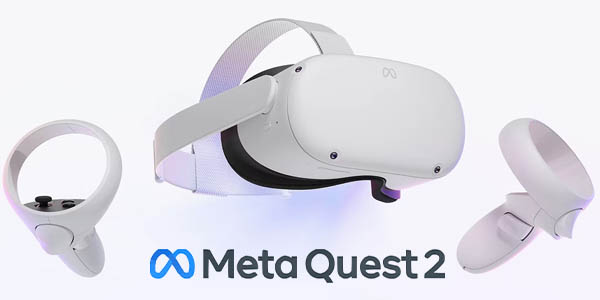
\includegraphics[width=0.8\textwidth]{../img/memoria/metaquest_2.jpg}
	\caption[Imagen de las gafas metaquest 2]{Gafas Meta Quest 2. Imagen extraída de ~\cite{metaquest2025}}
	\label{img:metaquest2}
\end{figure}

Las gafas Meta Quest 2 permiten una experiencia inmersiva sin necesidad de conexión a un ordenador externo, lo que facilita su uso en entornos clínicos y domésticos, aportando flexibilidad y autonomía al paciente durante las sesiones de rehabilitación. 

El dispositivo cuenta con dos controladores inalámbricos que permiten una interacción natural mediante detección de movimientos y pulsaciones, esenciales para la manipulación de los puzles y la navegación en el entorno virtual. Además, su sistema de seguimiento \textit{inside-out} utiliza cámaras integradas para detectar la posición y orientación de la cabeza y las manos del usuario, eliminando la necesidad de estaciones base externas.

Para el desarrollo y pruebas se ha empleado un ordenador personal compatible con las exigencias de Unreal Engine y la transmisión vía \textit{Link} para conectar las Meta Quest 2 al entorno de desarrollo cuando ha sido necesario.

La elección de este \textit{hardware} se ha basado en la disponibilidad del mismo para ser utilizado durante el desarrollo.

\subsection{Resumen de herramientas y técnicas empleadas}
En la tabla~\ref{tab:herramientas} se recogen las principales herramientas utilizadas durante el desarrollo del proyecto. Cada una de ellas ha sido seleccionada por su adecuación a los requisitos técnicos del entorno de \textit{realidad virtual}, facilitando tanto la implementación de la lógica de interacción como la organización del código, la documentación y la prueba del sistema. A continuación, se describe brevemente el propósito de cada herramienta y su papel en el flujo de trabajo del desarrollo.

\begin{table}[p]
    \centering
    \caption{Herramientas empleadas en el desarrollo del proyecto}
    \label{tab:herramientas}
    \begin{tabular}{|p{4.5cm}|p{9.5cm}|}
        \hline
        \textbf{Herramienta} & \textbf{Descripción} \\
        \hline
        \textbf{Unreal Engine 5} & Motor gráfico empleado para el desarrollo del entorno virtual interactivo en \textit{realidad virtual}. \\
        \hline
        \textbf{Plantilla VR de UE5} & Plantilla base integrada en Unreal Engine para VR, utilizada como punto de partida para la lógica de interacción y locomoción. \\
        \hline
        \textbf{Blueprints} & Sistema de scripting visual de Unreal Engine que ha permitido desarrollar lógica de juego sin necesidad de código en \textit{C++}. \\
        \hline
        \textbf{Victory Plugin} & Plugin para \textit{Blueprints} que habilita la exportación de datos en formato \textit{CSV}, entre otras funcionalidades extendidas. \\
        \hline
        \textbf{OpenXR Plugin} & Complemento oficial de Unreal Engine que permite la integración multiplataforma con dispositivos XR, garantizando compatibilidad con visores como \textit{Meta Quest 2}. \\
        \hline
        \textbf{Blender} & Suite de creación 3D utilizada para ajustar y exportar modelos 3D al formato compatible con Unreal Engine. \\
        \hline
        \textbf{GitLab} & Plataforma de control de versiones empleada para la gestión del código y la colaboración durante el desarrollo del proyecto. \\
        \hline
        \textbf{LaTeX} & Sistema de preparación de documentos científicos utilizado para redactar la memoria del proyecto. \\
        \hline
        \textbf{Meta Quest Link} & Herramienta para vincular las Meta Quest 2 a un PC durante el desarrollo y pruebas del entorno VR. \\
        \hline
    \end{tabular}
\end{table}

La Tabla~\ref{tab:tecnicas} presenta un resumen de las principales técnicas empleadas durante el desarrollo del proyecto. Estas técnicas han sido seleccionadas con el objetivo de asegurar una estructura de trabajo eficiente, centrada en la calidad del software, la satisfacción del usuario final y la facilidad de mantenimiento. Cada una de ellas contribuye a diferentes fases del ciclo de vida del desarrollo, desde la planificación hasta la verificación del sistema.

\begin{table}[p]
    \centering
    \caption{Técnicas empleadas en el desarrollo del proyecto}
    \label{tab:tecnicas}
    \begin{tabular}{|p{4.5cm}|p{9.5cm}|}
        \hline
        \textbf{Técnica} & \textbf{Descripción} \\
        \hline
        \textbf{Metodología ágil \textit{Scrum}} & Técnica de gestión del desarrollo basada en iteraciones cortas denominadas \textit{sprints}, con planificación, revisión y retrospectiva para mejorar el proceso de forma incremental. \\
        \hline
        \textbf{Programación modular} & División del sistema en módulos funcionales independientes y reutilizables, facilitando el mantenimiento, la escalabilidad y las pruebas unitarias. \\
        \hline
        \textbf{Diseño centrado en el usuario (DCU)} & Técnica que prioriza las necesidades, capacidades y limitaciones del usuario final durante todo el proceso de diseño e implementación. \\
        \hline
        \textbf{Control de versiones con \textit{Git}} & Gestión del código fuente mediante una herramienta distribuida para registrar cambios y mantener trazabilidad del desarrollo. \\
        \hline
        \textbf{Pruebas de sistema manuales} & Aplicación de una técnica de verificación funcional mediante ejecución directa de escenarios de uso en el entorno real, validando el comportamiento del sistema con distintos perfiles de usuario. \\
        \hline
    \end{tabular}
\end{table}